\documentclass[12pt]{article}
\usepackage{graphicx}
\usepackage{float}
\usepackage{amsmath}
\usepackage{sidecap}
\usepackage{fullpage}
\usepackage{hyperref}
\usepackage{listings}
\usepackage{latexsym}
\usepackage{color}
\usepackage{tikz}
\usetikzlibrary{shapes,arrows, matrix, positioning, fit}

% Java code with lstlisting
\definecolor{dkgreen}{rgb}{0,0.6,0}
\definecolor{gray}{rgb}{0.5,0.5,0.5}
\definecolor{mauve}{rgb}{0.58,0,0.82}

\lstset{frame=tb,
    language=Java,
    aboveskip=3mm,
    belowskip=3mm,
    showstringspaces=false,
    columns=flexible,
    basicstyle={\small\ttfamily},
    numbers=none,
    numberstyle=\tiny\color{gray},
    keywordstyle=\color{blue},
    commentstyle=\color{dkgreen},
    stringstyle=\color{mauve},
    breaklines=true,
    breakatwhitespace=true
    tabsize=3
}

\title{CIS4301 Notes}
\author{Ryan Roden-Corrent}
\date{\today}

\begin{document}
\setlength\parindent{0pt}
% Tikz general settings
\tikzstyle{relation} = [diamond, draw, fill=blue!20, text width=4em,
  text badly centered, node distance=3cm, inner sep=0pt]
\tikzstyle{attribute} = [draw, ellipse, fill=red!20, node distance=2.5cm,
  minimum height=2em]
\tikzstyle{entity} = [rectangle, draw, fill=blue!20, text width=5em,
  text centered, minimum height=4em]
\tikzstyle{relation-weak} = [diamond, double, draw, fill=blue!20, text width=4em,
  text badly centered, node distance=3cm, inner sep=0pt]
\tikzstyle{entity-weak} = [rectangle, draw, double, fill=blue!20, text width=5em,
  text centered, minimum height=4em]
\tikzstyle{line} = [draw, -]
\tikzstyle{arrow} = [draw, -latex', thick]
\tikzstyle{arrow-round} = [draw, -), thick]
\maketitle
\section{Relational Algebra}
See \url{http://cise.ufl.edu/class/cis4301sp14/slides/ra.ppt} for class slides
on this. These notes are mostly a condensed version of the slides, the slides
contain some nice table images to help you visualize the operations.

\subsection{What is Relational Algebra?}
\begin{description}
    \item[Operators] {most common actions you execute on relations}
    \item[Operands] {relations or variables that represent relations}
\end{description}

\subsection{Core Relational Algebra}
\begin{description}
    \item[Union,Intersection,Difference] {most common actions you execute on
        relations} 
    \item[Selection] {picking certain rows}
    \item[Projection] {picking certain columns}
    \item[Products/Joins] {compsitions of relations}
    \item[Renaming] {of relations and attributes}
\end{description}

\subsubsection{Selection}
$R1:=\sigma_c (R2)$\\
C is a condition that refers to attributes or R2\\
R1 is all tuples of R2 that satisfy C\\
\begin{center}
\begin{tabular}[H]{c||c}
  Relation Sells: & $JoeMenu := \sigma_{bar="Joe's"}(Sells):$\\
\begin{tabular}[H]{l|c|r}
  bar & beer & price\\
  \hline
  Joe's & Bud & 2.50\\
  Joe's & Miller & 2.75\\
  Sue's & Bud & 2.50\\
  Sue's & Miller & 3.00\\
\end{tabular}
&
\begin{tabular}[H]{l|c|r}
  bar & beer & price\\
  \hline
  Joe's & Bud & 2.50\\
  Joe's & Miller & 2.75\\
  Sue's & Bud & 2.50\\
  Sue's & Miller & 3.00\\
\end{tabular}
\end{tabular}
\end{center}


\subsubsection{Projection}
$R1 := \pi_L(R2)$\\
L is a list of attributes from R2's schema\\
R1 contains only the attributes of R2 listed in L (in the order they are
listed)\\
Set operation: removes duplicate tuples\\

\subsubsection{Extended Projection}
$R1 := \pi_L(R2)$\\
Like projection, but L can contain arbitrary expressions involving attributes.
Example: $\pi_{A+B->C,A,A}(R)$ will create a new table where the first column,
C, is the sum of A and B, and the next two columns A1 and A2 are copies of the
original A.

\subsubsection{Product}
$R3 := R1 X R2$
\begin{itemize}
    \item{pair each tuple t1 or R1 with each tuple t2 of R2}
    \item{Concatenation $t_1 t_2$ is a tuple of $R_3$}
    \item{Schema of R3 is the attributes of R1 and then R2, in order}
    \item{Beware attribute A of same name in R1 and R2: use R1.A and R2.A}
\end{itemize}
Example: $R3 := R1 X R2$\\
Duplicate column B, so use R1.B and R2.B to differentiate.

\subsubsection{Theta Join}
$R3 := R1 \Join_C R2$
Equivalent to taking the product $R1 X R2$ and applying $\sigma_C$ to the
result.\\
$R \Join_{\theta} S \equiv \sigma_{\theta}(R X S)$\\
C can be any boolean-values condition.

\subsubsection{Natural Join}
Remove duplicate columns, only return columns that naturally combine.
$R3 := R1 \Join R2$

\subsubsection{Renaming}
Gives a new schema to a relation.\\
$R1:= \rho_{R1(A_1,...,A_n)}(R2)$ or $R1(A_1,...,A_n) := R2$ (simplified
notation)\\
R1 is a relation with the same tuples as R2 but the attribtues $A_1,...,A_n$.

\subsection{Building Complex Expressions}
Combine operators with parentheses and precedence rules.\\
Three notations:\\
\begin{enumerate}
    \item{Sequences of assignment statements}
    \item{Expressions with several operators}
    \item{Expression trees}
\end{enumerate}
\subsubsection{Operator Precedence}
\begin{enumerate}
    \item{$[\sigma,\pi,\rho]$ (highest)}
    \item{$[X,\Join]$}
    \item{$\cap$}
    \item{$\cup$}
\end{enumerate}


\subsubsection{Expression Trees}
Leaves are operands (variables or constant relations).\\
Interior nodes are operators applied to children.\\
\textbf{Example:}\\

\begin{figure}[H]
\begin{tikzpicture}[node distance = 2cm, auto]
  \node (union) {$\cup$};

  \node [below left of=union] (l1) {$\rho_{R(name)}$};
  \node [below of=l1] (l2) {$\pi_{bar}$};
  \node [below of=l2] (l3) {$\sigma_{price<3 AND beer="bud"}$};
  \node [below of=l3] (l4) {$Sells$};

  \node [below right of=union] (r1) {$\pi_{name}$};
  \node [below of=r1] (r2) {$\sigma_{addr="Maple St."}$};
  \node [below of=r2] (r3) {$Bars$};

  \draw [<-] (union) -- (r1);
  \draw [<-] (r1) -- (r2);
  \draw [<-] (r2) -- (r3);
  \draw [<-] (union) -- (l1);
  \draw [<-] (l1) -- (l2);
  \draw [<-] (l2) -- (l3);
  \draw [<-] (l3) -- (l4);
\end{tikzpicture}
\caption{Find the names of all bars that are either on maple street or sell Bud
for less than \$3}
\end{figure}

\subsection{Relational Algebra on Bags}
A bag is like a set, but duplicate elements are allowed. SQL is a bag
language. Operations like projection are more efficient on bags than on sets.
\subsubsection{Bag Union}
Just add elements together, including duplicates.\\
$\{1,2,1\} \cup \{1,1,2,3,1\} = \{1,1,1,1,1,2,2,3\}$
\subsubsection{Bag Intersection}
Minimum number of duplicates in resulting set.\\
$\{1,2,1,1\} \cap \{1,2,1,3\} = \{1,1,2\}$
\subsubsection{Bag Difference}
Result contains all tuples in first relation that aren't in the second.\\
$\{1,2,1,1\} - \{1,2,3\} = {1,1}$
\subsubsection{Bag Laws != Set Laws}
Set union is \textbf{idempotent}, (result does not change if applied multiple
times.)\\
For a bag union, if x appears n times in S, then it appears 2n times in union.

\section{Why SQL?}
Say what to do rather than how to do it.
\begin{description}
    \item[SELECT]{desired attributes}
    \item[FROM]{one or more tables}
    \item[WHERE]{some condition holds}
\end{description}
\subsection{Example:}
Names of beers made by Anheuser-Busch:
\begin{lstlisting}[language=SQL]
  SELECT name
  FROM Beers
  WHERE manf = 'Anheuser-Busch'
\end{lstlisting}

\begin{table}[H]
  \begin{tabular}{|c|c|}
    \hline
    name & manf\\
    \hline
    Bud & Anheuser-Busch\\
    \hline
\end{tabular}
\end{table}

* indicates "all attributes in relation.
\begin{lstlisting}[language=SQL]
  SELECT name
  FROM Beers
  WHERE manf = 'Anheuser-Busch'
\end{lstlisting}
Try adding things to SELECT *

Rename \emph{name} to \emph{beer} using \textbf{AS}
\begin{lstlisting}[language=SQL]
  SELECT name AS beer, manf
  FROM Beers
  WHERE manf = 'Anheuser-Busch'
\end{lstlisting}

\begin{lstlisting}[language=SQL]
  SELECT bar, ber,
  price*114 AS PriceInYen
  FROM Beers
\end{lstlisting}

Using \textcolor{purple}{Likes(drinker, beer)}:
Put 'likes Bud' in attribute whoLikesBud
\begin{lstlisting}[language=SQL]
  SELECT drinker
    'likes Bud' AS whoLikesBud
    FROM Likes
    WHERE beer = 'Bud'
\end{lstlisting}

\subsection{Information Integration}
Each \textbf{Data warehouse} manages several subdatabases that each have multiple tables.\\

Example: Each bar has its own relation Menu(beer,price) tat we need to
integrate.
\begin{lstlisting}[language=SQL]
  SELECT 'Joe''s Bar', beer, price
  FROM Menu;
\end{lstlisting}
Do this for each bar to create a consistent schema, then take the Union.\\
\textbf{Note}: the repeated single quote is used to escape the nested quote.

\subsection{Complex Conditions}
Using \textcolor{purple}{Sells(bar, beer, price)}, find the price Joe charges
for Bud.  
\begin{lstlisting}[language=SQL]
  SELECT price
  FROM Sells
  WHERE bar = 'Joe''s Bar' AND beer = 'Bud';
\end{lstlisting}

\subsection{Patterns}
Usable on \textbf{VARCHAR}. Useable on \textbf{DATE, INT}? Maybe.
\begin{verbatim}
  <Attribute> LIKE <pattern>
  <Attribute> iLIKE <pattern>   --case insensitive like
  <Attribute> NOT LIKE <pattern>
\end{verbatim}

\begin{description}
    \item[\%] {means any string}
    \item[\_] {means any character}
\end{description}

Example: choose numbers with two digits
\begin{lstlisting}[language=SQL]
  FROM NUMBERS
  WHERE number LIKE "__"
\end{lstlisting}
Example: choose numbers with at least two digits
\begin{lstlisting}[language=SQL]
  FROM NUMBERS
  WHERE number LIKE "__%"
\end{lstlisting}
Find drinkers with phone number starting with 555.
\begin{lstlisting}[language=SQL]
  SELECT name
  FROM Drinkers
  WHERE phone LIKE '%555-_ _ _ _';
\end{lstlisting}

\subsection{NULL Values}
NULL could mean:
\begin{description}
    \item[Missing Value]{we know it exists but dont have value}
    \item[Inapplicable]{e.g. spouse of unmarried person}
\end{description}

NULLs can be tricky, try to avoid if possible.\\
\subsubsection{3-valued logic}
TRUE = 1, FALSE = 0, UNKNOWN = 1/2\\
AND = MIN, OR=MAX, NOT(x) = 1-x\\
Ex:
\begin{verbatim}
TRUE AND (FALSE OR NOT(UNKNOWN)) = MIN(1, MAX(0, (1-1/2)))
\end{verbatim}
Start on innermost paren and change truth values to numeric values.
E.g. NOT(UNKNOWN) = (1-1/2)

\subsubsection{Surprising Example}
\begin{table}[H]
  \begin{tabular}{|c|c|c|}
    \hline
    bar & beer & price\\
    \hline
    Joes & Bud & NULL\\
    \hline
\end{tabular}
\end{table}

\begin{lstlisting}[language=SQL]
  SELECT bar
  FROM Sells
  WHERE price < 2.00 OR price >= 2.00;
\end{lstlisting}
The comparisons become UNKNOWN because they are undefined for NULL.\\
Result is 
\begin{verbatim}
  NULL OR NULL
  Max(1/2,1/2) = 1/2
\end{verbatim}
Expected to get everything, got nothing

\subsection{Multirelation Queries}
Distinguish between attributes of same name by 
"relation.attribute"

\subsubsection{Examples}
Using \textcolor{purple}{Likes(drinker,beer), Frequents(drinker, bar)},
find the beers liked by at least one person who frequents Joe's.
\begin{lstlisting}[language=SQL]
  SELECT beer
  FROM Likes, Frequents
  WHERE Bar = 'Joes' AND
    Frequents.drinker = 
      Likes.drinker;
\end{lstlisting}
A theta join $\Join_{=}$ is used to equate the drinker attribute from each table.
Can be done in any order.\\
For example:

\begin{tikzpicture}[node distance = 2cm, auto]
  \node (c0) {$\pi_{beer}$};
  \node [below of = c0] (c1) {$\Join_{drinker=drinker}$};
  \node (r2) [below right of = c1] {$\sigma_{bar='joes'}$};
  \node (r3) [below of = r2] {Frequents};
  \node (l2) [below left of = c1] {Likes};

  \draw [<-] (l2) -- (c1);
  \draw [<-] (c1) -- (r2);
  \draw [<-] (r2) -- (r3);
  \draw [<-] (c0) -- (c1);
\end{tikzpicture}


\section{Multirelational Queries}
\subsection{Joining Two Relations}
Find the beers liked by at least one person who frequents Joe's
\begin{lstlisting}[language=SQL]
  SELECT beer
  FROM Likes, Frequents
  WHERE bar = 'Joes' AND
    Frequents.drinker = 
      Likes.drinker;
\end{lstlisting}
Same as a $\Join_{Frequents.drinker and Likes.drinker}$

\subsection{Self-Join}
Get all pairs of beers that have same manufacturer and a different name.
\begin{lstlisting}[language=SQL]
  SELECT b1.name, b2.name
  FROM Beers b1, Beers b2 --avoid naming conflicts
  WHERE b1.manf = b2.manf AND
    b1.name < b2.name;
\end{lstlisting}
Why use \fbox{$<$} instead of \fbox{$<>$}? $<$ will order the results and get
rid of duplicates.

\subsection{Subqueries}
A parenthisized SELECT-FROM-WHERE statement

\begin{lstlisting}[language=SQL]
  SELECT beer
  FROM Likes, (SELECT drinker
    FROM Frequents                  --create a table of drinkers who frequent joes
    WHERE bar = 'Joes') AS JD       --and call that table JD
  WHERE Likes.Drinker = JD.drinker  --now operate on that table
\end{lstlisting}

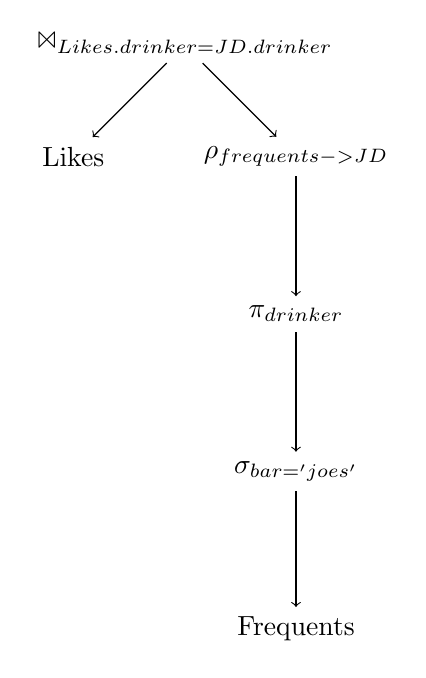
\begin{tikzpicture}[node distance = 2cm, auto]
  \node (c0) {$\Join_{Likes.drinker=JD.drinker}$};

  \node (r3) [below right of = c0] {$\rho_{frequents->JD}$};
  \node (r2) [below of = r3] {$\pi_{drinker}$};
  \node (r1) [below of = r2] {$\sigma_{bar='joes'}$};
  \node (r0) [below of = r1] {Frequents};

  \node (l0) [below left of = c0] {Likes};

  \draw [<-] (r0) -- (r1);
  \draw [<-] (r1) -- (r2);
  \draw [<-] (r2) -- (r3);
  \draw [<-] (r3) -- (c0);
  \draw [<-] (l0) -- (c0);
\end{tikzpicture}

\subsubsection{Query + Subquery Solution}
Get the the bars where Miller is sold for the same price as bud at Joe's.
\begin{lstlisting}[language=SQL]
  SELECT bar
  FROM Sells
  WHERE beer = 'Miller' AND
    price = (SELECT price   --get the price from a subquery
    FROM Sells
    WHERE bar = 'Joes'
      AND beer = 'Bud'
      LIMIT 1);       --Make sure you only get a single value
\end{lstlisting}
There is a runtime error if the subquery returns more than one value (hence the
use of LIMIT).

\subsubsection{IN}
Get the name and manufacturer of each beer that Fred likes.
\begin{lstlisting}[language=SQL]
  SELECT *
  FROM Beers
  WHERE name IN (SELECT beer
    FROM Likes
    WHERE drinker = 'Fred');
\end{lstlisting}

\subsubsection{EXISTS}

Correlated subquery: 
Walk one-by-one through tuples.
At each tuple, perform the WHERE check.
b1 refers to the tuple being checked.
\begin{lstlisting}[language=SQL]
  SELECT name
  FROM Beers b1
  WHERE NOT EXISTS (  --only true if subquery returns empty set
    SELECT *    --get manufacturers who have only one beer
    FROM Beers
    WHERE manf = b1.manf AND
      name <> b1.name); --returns a tuple (manf, beer)
\end{lstlisting}

\textbf{EXISTS} looks at a table and finds out if the table returns any values.
Either returns $\emptyset$ or a table of results. \textbf{NOT EXISTS}(query)
returns true only if the result of query is $\emptyset$.
Internal query returns beers where the manufacturer is 'Bud' and the name is not
'Lite'.

\subsubsection{ANY}
$x = ANY (subquery)$ checks if  x equals at least one tuple in the subquery.
\subsubsection{ALL}
$x <> ALL(subquery)$ is true iff x is not equal to any tuple in the subquery.

\subsubsection{DISTINCT}
Remove duplicates

\begin{lstlisting}[language=SQL]
  SELECT x,y
\end{lstlisting}

\subsection{Union, Intersect, Difference}
Set operators. Require that arguments have same schema. 

\section{Bag Semantics}
Just add ALL to any of the set operators e.g. UNION ALL.
\begin{description}
  \item[$\delta$]{remove duplicate tuples}
  \item[$\tau$]{sort tuples}
  \item[$\gamma$]{grouping and aggregation}
\end{description}

Sorting\\
$R1 := \tau_L(R2)$\\
L is a list of attributes to list by, listed in order of priority.

\subsection{Grouping}
$R1 := \gamma_L(R2)$\\
\begin{tabular}{|c|c|c|}
  \hline
  A & B & C\\
  \hline
  1 & 2 & 3\\
  \hline
  4 & 5 & 6\\
  \hline
  1 & 2 & 5\\
  \hline
\end{tabular}
$gamma_{A,B,AVG(C)->X}(R) = ??$\\
First, group R by A and B.\\ 
\begin{tabular}{|c|c|c|}
  \hline
  A & B & C\\
  \hline
  1 & 2 & 3\\
  \hline
  1 & 2 & 5\\
  \hline
  4 & 5 & 6\\
  \hline
\end{tabular}\\
Then, average C within groups\\
\begin{tabular}{|c|c|c|}
  \hline
  A & B & C\\
  \hline
  1 & 2 & 4\\
  \hline
  4 & 5 & 6\\
  \hline
\end{tabular}

\subsection{Outerjoin}
\newsavebox\outerjoinexone
\savebox\outerjoinexone {
\begin{tabular}{|c|c|}
  \hline
  A & B\\ 
  \hline
  1 & 2\\
  \hline
  4 & 5\\
  \hline
\end{tabular}
}
\newsavebox\outerjoinextwo
\savebox\outerjoinextwo {
\begin{tabular}{|c|c|}
  \hline
  B & C\\ 
  \hline
  2 & 3\\
  \hline
  6 & 7\\
  \hline
\end{tabular}
}
\newsavebox\outerjoinexthree
\savebox\outerjoinexthree {
\begin{tabular}{|c|c|c|}
  \hline
  A & B & C\\ 
  \hline
  1 & 2 & 3\\
  \hline
  1 & 2 &  \\
  \hline
    & 6 &  7\\
  \hline
  4 & 5 &  \\
  \hline
    & 2 & 3\\
  \hline
  4 & 5 &  \\
  \hline
    & 6 &  7\\
  \hline
\end{tabular}
}
\newsavebox\outerjoinexfour
\savebox\outerjoinexfour {
\begin{tabular}{|c|c|c|}
  \hline
  A & B & C\\ 
  \hline
  1 & 2 & 3\\
  \hline
  4 & 5 & NULL\\
  \hline
  NULL & 6 & 7\\
  \hline
\end{tabular}
}

\begin{figure}[H]
\begin{tikzpicture}[node distance = 4cm, auto]
  \node (d)  {\usebox{\outerjoinexfour}};
  \node (c) [above of = d]  {\usebox{\outerjoinexthree}};
  \node (b) [above right of = c]  {\usebox{\outerjoinextwo}};
  \node (a) [above left of = c]  {\usebox{\outerjoinexone}};

  \path [arrow] (a) -| (c);
  \path [arrow] (b) -| (c);
  \path [arrow] (c.south) -| (d);
\end{tikzpicture}
\end{figure}

\subsubsection{JOIN Modifiers}
R OUTER JOIN S is the core of an outerjoin. Can be modified by
\begin{itemize}
    \item{NATURAL before JOIN}
\end{itemize}

\subsection{Aggregations}
Not operators of relational algebra, apply to an entire column.\\
Builtins: SUM, AVG, COUNT, MIN, MAX\\
Can define your own in postgres.\\
NOTE: NULL's are ignored in Aggregations.
\subsubsection{Return a table with the single column AVG(Price).}
\begin{lstlisting}[language=SQL]
  SELECT AVG(price)
  FROM Sells
  WHERE beer = 'Bud';
\end{lstlisting}

\subsubsection{Return number of distinct prices for bud beers}
\begin{lstlisting}[language=SQL]
  SELECT COUNT(DISTINCT price)
  FROM Sells
  WHERE beer = 'Bud';
\end{lstlisting}

\subsection{Grouping}
Follow SELECT-FROM-WHERE by GROUP-BY and a number of attributes

\subsubsection{Get the Average price for each beer}
\begin{lstlisting}[language=SQL]
  SELECT Beer, AVG(price)
  FROM Sells
  GROUP BY beer;
\end{lstlisting}
Anything in GROUP BY must also be in SELECT.\\
In relational algebra: 
$\gamma_{beer,AVG(price)}$\\
Result: 
\begin{tabular}{|c|c|}
  \hline
  beer & AVG(price)\\ 
  \hline
  bud & 2.33\\ 
  coors & 4.00\\ 
  ... & ...\\
\end{tabular}

\subsubsection{Average Age by Gender}
\begin{lstlisting}[language=SQL]
  SELECT gender, AVG(age)
  FROM People
  GROUP BY age;
\end{lstlisting}

Result:
\begin{tabular}{|c|c|}
  \hline
  gender & AVG(age)\\ 
  \hline
  M & 24\\ 
  F & 23\\ 
  \hline
\end{tabular}

\subsubsection{Illegal Example}
\begin{lstlisting}[language=SQL]
  SELECT bar, MIN(price)
  FROM Sells
  GROUP BY beer = 'Bud';
\end{lstlisting}

\subsection{Having}
Get only certain rows based on a condition.
\subsubsection{Get average age only for genders where it is greater than 24}
\begin{lstlisting}[language=SQL]
  SELECT gender, AVG(age)
  FROM People
  GROUP BY gender
  HAVING AVG(age) > 23
\end{lstlisting}
Result:
\begin{tabular}{|c|c|}
  \hline
  gender & AVG(age)\\ 
  \hline
  M & 24\\ 
  \hline
\end{tabular}

\end{document}
